\chapter{Задачі, напрямки та методи захисту інформації.
    Поняття про криптографічний захист інформації}
\section{Області застосування, мета, методи захисту інформації}
Протягом свого існування людство пережило декілька інформаційних революцій:
створення і розвиток мов, винахід писемності, винахід та широке застосування
друкарства, створення комп’ютера та новітніх електронних технологій, що
радикально змінили суспільство в усіх галузях, на всіх рівнях  суспільного
розвитку. Кількість інформації, що була доступна та використовувалась, постійно
зростала, а за періоди інформаційних революцій --- на декілька порядків.
Володіння інформацією і в минулому і нині давало можливість досягти швидкого
розвитку і успіху у різних галузях як у глобальному масштабі, так і в
конкретних справах. Сьогодні світ переживає період, коли накопичено колосальний
об’єм знань, що  дозволяє перейти до здійснення справді революційних
технологічних рішень. Основою розвитку  нині може бути, перш за все, процес
пізнання, і він посильний тільки високоосвіченому суспільству, в якому праця
приймає все більш інтелектуальні форми. Технологіям майбутнього потрібні широко
освічені люди, які здатні орієнтуватися в нових умовах дійсності, що стрімко
змінюється.

Однією з галузей, що  найбільш динамічно  змінюються  протягом останніх
десятиліть, є технології електронної обробки інформації, телекомунікацій,
комп’ютерних мереж, технології захисту інформації.

В Україні широкий попит на методи і засоби захисту інформації почав виявлятися у
другій половині 80-х років ХХ ст. З часом виникла нагальна потреба використання
криптографічних та технічних методів захисту також у приватному секторі.
Сьогодні велика кількість конфіденційної інформації передається в електронному
вигляді, на електронних носіях, між ЕОМ звичайними лініями зв’язку. Інформація
може продаватися та купуватися, мати ціну, що незрівнянно перевищує ціну
матеріального носія. Часто володіння інформацією дає переваги, ціну яких
неможливо підрахувати, наприклад, у військовій справі. Термін збереження
секретності інформації може коливатися від декількох годин до багатьох
десятиліть. Тому вкрай потрібні спеціалісти, які володіють  криптографічними,
технічними, комплексними методами захисту, знають відповідні стандарти, здатні
використовувати (або розробляти) програмне й апаратне забезпечення для
гарантування таємності та цілісності конфіденційної інформації. Криптографічні
методи захисту вважаються одними з найбільш надійних та ефективних. 

\begin{itemize}
    \item{Області застосування захисту інформації
        (відповідно --- види таємниці):}
        \begin{multicols}{2}
            \begin{enumerate}
                \item Військова;
                \item Дипломатична;
                \item Фінансова;
                \item Банківська;
                \item Комерційна;
                \item Промислова;
                \item Наукова;
                \item Юридична;
                \item Медична;
                \item Особиста таємниця.
            \end{enumerate}
        \end{multicols}
    \item{Мета і головні задачі захисту інформації:}
        \begin{enumerate}
            \item Конфіденційність (секретність) інформації;
            \item Цілісність інформації;
            \item Автентичність інформації;
            \item Доступність інформації.
        \end{enumerate}
    \item{Напрямки, аспекти, методи і засоби захисту інформації:}
        \begin{enumerate}
        \item Юридичні, правові;
        \item Методично-нормативні;
        \item Організаційні;
        \item Безпосередні (фізичні);
        \item Технічні --- захист від витоку  по технічним каналам:
            \begin{enumerate}
                \item електромагнітному
                \item оптичному
                \item акустичному
                \item віброакустичному;
        \end{enumerate}
        \item Стеганографічні;
        \item Криптографічні. Методи математичного захисту інформації; 
        \item Методи квантової криптографії; 
        \item Морально-етичні норми.  
    \end{enumerate}
\end{itemize}
\section{Перші поняття криптографічного  захисту інформації}

\begin{definition}[Криптографічний захист інформації]
    Криптографічний захист інформації --- це різновид
    захисту інформації, який реалізується за допомогою криптографічних перетворень,
    спеціальних ключових даних з метою приховування та відновлення змісту
    інформації, підтвердження достовірності, авторства, запобігання
    несанкціонованому використанню тощо.
\end{definition}

\begin{definition}[Криптографічне перетворення]
    Криптографічне перетворення --- це перетворення
    інформації відповідно до певних правил (логічних, математичних) з метою
    забезпечення функціонування криптографічних протоколів.
\end{definition}

\begin{definition}[Криптографічний ключ]
    Криптографічний ключ --- це параметр, який
    використовується в криптографічному алгоритмі для вибору конкретного
    криптографічного перетворення; ключі можуть бути таємними або відкритими.
\end{definition}

\begin{definition}[Криптографічний протокол]
    Криптографічний протокол --- це послідовність
    узгоджених дій згідно з деякими правилами, у відповідності з якими відбувається
    обмін інформацією між сторонами або учасниками протоколу та її перетворення з
    використанням криптографічних методів і засобів.  Простий приклад
    криптографічного протоколу – це зашифрування та розшифрування повідомлення.
\end{definition}

\begin{definition}[Криптографія]
    Криптографія --- науково-технічна дисципліна, яка
    вивчає принципи, методи і засоби криптографічного захисту інформації і
    інформаційних технологій, предметом якої є розробка криптографічних систем.
\end{definition}

\begin{definition}[Криптоаналіз]
    Криптоаналіз --- це науково-технічна дисципліна, яка
    вивчає методи, способи і засоби аналізу криптографічного захисту інформації:
    криптографічних систем, криптографічних алгоритмів, протоколів з метою знайти
    способи їх розкриття без знання секретних ключів і, можливо, будови
    криптосистем, знайти способи несанкціонованого доступу, підробки даних тощо.
    Криптоаналіз оцінює складність таких способів  розкриття (злому) і стійкість
    криптографічного захисту інформації. Фахівця, який займається криптоаналізом
    будемо називати криптоаналітиком.
\end{definition}

\begin{definition}[Криптологія]
    Криптологія за найбільш поширеною сучасною
    термінологією, об'єднує в собі дисципліни криптографію і
    криптоаналіз.
\end{definition}

\begin{remark}
    Не всі  країни дотримуються останньої термінології щодо
    дисциплін. Так, наприклад, в Росії назва „криптографія” об’єднує в собі власне
    криптографію (криптосинтез) у вище наведеному розумінні і криптоаналіз, а
    криптологія розглядається як галузь криптографії, що вивчає математичні моделі
    криптографічних систем, і також поділяється на криптосинтез та криптоаналіз.
\end{remark}
\section{Етапи розвитку технологічних засобів  криптографії}
\begin{enumerate}
    \item ``Ручна'' криптографія (із давнини до середини-кінця XIX століття)

        Основні види шифрів --- заміни і перестановки.

        \begin{figure}[hb]
            \centering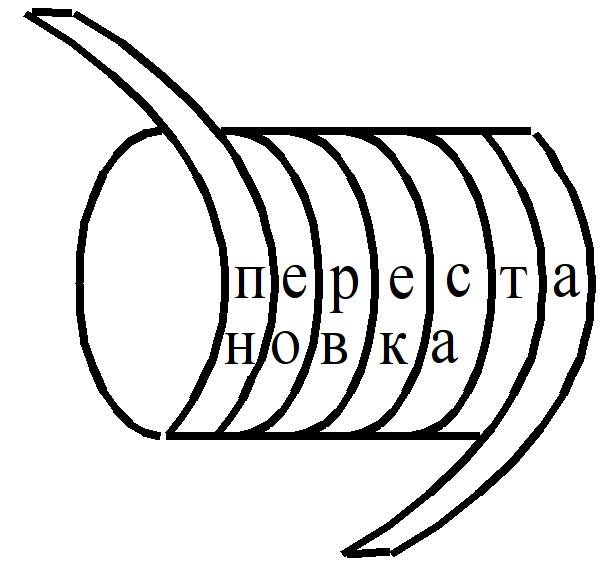
\includegraphics[width=1.0in]{crypt-img/crypt-img1.png}
            \caption{Шифр Скитала}\label{scitalCipher}
        \end{figure}

        Перший шифр перестановки,
        застосування якого зафіксоване у військовій справі,
        (Спарта, V ст. до н.е.) – шифр Скитала (рис. \ref{scitalCipher}).
        Таємний ключ – діаметр барабана.

        \begin{figure}[hb]
            \centering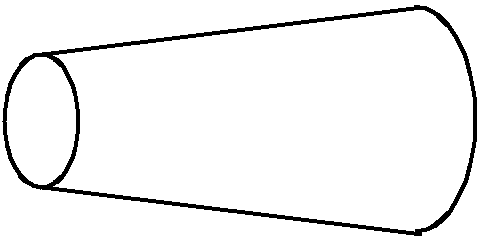
\includegraphics[width=1.0in]{crypt-img/crypt-img2.png}
            \caption{Засіб криптоаналізу шифру Скитала}\label{scitalAnalysis}
        \end{figure}

        Для  шифрування на стрічці, що намотувалась на барабан (скитал),
        писалось вздовж барабана повідомлення.
        Після знімання з барабану на стрічці була зовні
        випадкова послідовність літер – шифроване повідомлення.
        Криптоаналіз шифру Скитала запропонував Арістотель
        за допомогою барабана змінного діаметру (рис. \ref{scitalAnalysis}):
        якщо на намотаній на нього стрічці з шифрованим повідомленням у
        деякому місці вгадувались якісь частини слів,
        то цьому місцю відповідав діаметр справжнього барабану. 

        Прикладом шифру заміни є шифр Цезаря --- заміна кожної букви
        повідомлення на букву  циклічно віддалену
        в алфавіті на фіксоване число позицій.
    \item Застосування телеграфу для шифрування і кодування (з середини XIX ст.)
    \item Використання механічних машин (кінець XIX ст. – 20і роки XX ст.)
    \item Електромеханічні машини (з 20-х років XX ст. – середина XX ст.)

        Приклад --- ENIGMA --- основна шифрувальна машина Вермахту
        у Другій світовій війні.
    \item Електронні машини (з кінця 40-х років XX ст.)
    \item Напівпровідникові криптосистеми
    \item Криптосистеми, засновані на мікросхемах
    \item Використання комп'ютерної техніки для криптографічного захисту
    \item Квантова криптографія
\end{enumerate}

\section{Про розвиток теоретичної криптографії}

До епохи Відродження криптографією займалися, можна сказати, не професіонали.
Найчастіше шифри уявляли  собою деякі головоломки. Але слід зазначити, що іноді
винаходилися шифри, які не були розкриті на протязі  100 і навіть більше років!
Хоча за сучасними  поняттями,  враховуючи залучення до криптоаналізу ЕОМ,
загалом це були  слабкі, нестійкі шифри.

Велике просування в криптографії відбулося після залучення до вирішення її
проблем  відомих математиків періоду відродження, серед яких  були Ф. Вієт, Д.
Кардано та ін. Пізніше почали створюватись спеціалізовані державні служби
шифрування і дешифрування (розкриття). Такі служби створили, наприклад,
Кромвель у Англії, кардинал Рішельє у Франції, Петро I  в Росії. 

У 1883 році була опублікована  книга Керкгоффа «Військова криптографія», в якій 
були вперше сформульовані деякі вимоги до криптосистем, правила щодо утворення,
експлуатації, стійкості  криптографічних пристроїв. Частина цих правил і зараз
вважаються обов'язковими. 

Наукою у повному розумінні цього слова теоретичну  криптографію стали визнавати
з 1949 року після публікації у відкритому друці  статті К. Шеннона ``Теорія
зв'язку в секретних системах''. А з 1976 року завдяки ідеям
статті  Діффі і Хеллмана ``Нові напрямки в криптографії'' почався новий  етап у
розвитку  криптографії – застосування криптосистем з відкритим ключем, яке дало
можливість успішно вирішити низку назрілих  проблем криптографічного захисту
інформації.

\section{Класифікація сучасних  криптосистем}

\begin{enumerate}
    \item \textit{Симетричні (одноключові, з секретним ключем).}
        Підрозділяються на блокові й потокові.
        У відправника та одержувача повідомлення один і той самий
        секретний ключ, вони знаходяться у рівних (симетричних) умовах,
        можуть як зашифрувати повідомлення так і  розшифрувати
        за допомогою таємного ключа.
    \item \textit{Асиметричні (двохключові, з відкритим ключем, із
        загальнодоступними ключами).}
        Відомі з 1976 року, активно використовуються на практиці з 1978 року.
        У найпростішому випадку мають два ключі: один (відкритий)
        --- у відправника для шифрування, інший --- у одержувача (секретний) для
        розшифрування.
    \item \textit{Квантові} (знаходяться у стадії експерименту та розвитку)
\end{enumerate}

\section{Контрольні питання}
\begin{enumerate}
    \item Які  мета та задачі захисту інформації?
    \item Назвіть напрямки та методи захисту інформації.
    \item Що таке криптографічний ключ?
    \item З яких частин складається криптологія?
    \item Чи були відомі способи захисту інформації шифруванням до нашої ери?
    \item Коли використовувались роторні шифрувальні машини?
    \item Яка дата вважається початком розвитку криптографії
        з відкритим  ключем?
    \item Чим відрізняються симетричні криптосистеми від асиметричних?
\end{enumerate}
